\documentclass{sig-alternate}
\usepackage{verbatim}
\usepackage{array}
\usepackage{caption}
\usepackage{subcaption}

\newtheorem{definition}{Definition}
\begin{document}
%
% --- Author Metadata here ---
\conferenceinfo{SIGIR}{'2016 Pisa, Italy}

\title{Detecting significant events in news corpora}

\maketitle
\begin{abstract}
Retrospective event identification is the task of identifying and summarizing significant events in time-stamped corpora. In this short paper, we present a simple unsupervised method for identifying significant events in a news corpus based on feature temporal mutual information ($I_t$) and non-negative matrix factorization (NMF). We introduce a preliminary test collection and evaluation methodology that can be used for future comparative research. We compare our method to a latent Dirichlet allocation (LDA) approach to better understand the differences between events and topics.

\end{abstract}

% A category with the (minimum) three required fields
\category{H.3.3}{Information Search and Retrieval}{}

\terms{}

\keywords{Event detection}

\section{Introduction}

Imagine a Wikipedia editor creating a `year' page (e.g., https://en.wikipedia.org/wiki/1988\#Events) containing a list of important events that occurred during that year. Given a corpus of news articles (or other timestamped collection), it should be possible to show the editor a list of major events that were reported during the time period to facilitate the creation or validation of these pages. Such a system might rank the events by importance, provide estimated dates of event occurrence, and a ranking of candidate Wikipedia pages that describe the associated event. 

In this short paper, we present a novel method for retrospective event identification in news corpora based on temporal mutual information \cite{Teng2008} and non-negative matrix factorization \cite{Lee2001}. We also introduce a preliminary test collection and evaluation methodology based on Wikipedia that can be used for future comparative research.  As far as we know, we are the first to propose a method for comparative evaluation in this type of retrospective event identification task.

Following \cite{Weng2011}, we compare the results of our method to an LDA baseline. For the purpose of retrospective event identification, our model consistently outperforms the baseline.

This short paper is organized as follows. In Section 2 we review the concept of significant events followed by a summary of related work in Section 3. In Sections 4 and 5 we introduce our model and the LDA baseline model. Section 6 describes the evaluation methodology and test collection. Section 7 summarizes the results followed by conclusions and next steps in Section 8.

\section{What is an event?}

The concepts of `event detection' or `event extraction' are common in the information retrieval and natural language processing literature. In this paper, we are concerned with the identification of large-scale events as reported in historical news corpora. A number of studies have used the concepts of ``significant,'' ``seminal,'' or ``newsworthy'' events to describe such large-scale events.  Our notion of event is most closely related to the ``seminal events'' of the Topic Detection and Tracking (TDT) task, although the task itself is quite different. Examples of large-scale events include major elections, natural disasters, political revolutions, wars, and acts of violence.


\section{Related Work}

Recent studies in retrospective event identification apply feature-centric models \cite{Yi, Fung2005, Chen2009, Teng2008, Weng2011} that first identify interesting terms (or features) which are subsequently grouped or combined to represent events. 

For example, Fung et al \cite{Fung2005} identify temporally interesting features using a series of binomial distributions. The terms are subsequently combined  into events using a cost-minimization approach that balances the similarity of the temporal distributions of terms and the co-occurrence of terms in documents. 

He, Chang and Lim \cite{He2007} use spectral analysis to identify interesting features in text corpora. Features are grouped into events using a cost-minimization approach that combines the similarity of the temporal distributions using KL divergence and co-occurrence of terms in documents. 

Weng and Lee \cite{Weng2011} use wavelet analysis to identify interesting features and then apply graph partitioning to a graph with terms as nodes and the cross-correlation of term time-series as edge weights. This approach does not account for term co-occurrence in documents.

Also related to the current study is research in latent semantic analysis (LSA) \cite{Deerwester1990, Hofmann1999} and topic modeling \cite{Blei2003}.  Event models can be seen as a special type of temporally-constrained topic models. Our approach is akin to the factor-based LSA approach, but we anticipate expanding this work to a generative probabilistic framework in the future.  




\section{Event detection model (TMINMF)}

Each of the feature-centric models described above includes two basic steps. The first is to identify terms or features that are indicative of an event in the corpus, generally using time-series methods. The second is to combine terms generated by the same underlying event into event models.  This is usually done by balancing temporal similarity (e.g., time series correlation) with term co-occurrence in documents.

In this study, we identify temporally interesting terms using the first-order autocorrelation (ACF) of the term time series \cite{Jones2007}. We then calculate the temporal mutual information between the top $K$ terms based on ACF and apply non-negative matrix factorization (NMF) to identify latent factors. We interpret the resulting factors as events. The basic process is defined as follows:

First, we construct a temporal index from the document collection that consists of time series for each term in the vocabulary at a particular interval (e.g., hour, day, week):
\begin{definition}
 \text{ \normalfont Feature time series. }
 The time series of a feature f is defined as the sequence:
\[
y_f = [y_f(1), y_f(2), ..., y_f(T)],
\]
where each element $y_f(t)$ is a measure of feature f at time t. For this paper, we use the simple document frequency:
\[
	y_f(t) = DF_f(t)
\]
where $DF_f(t)$ is the number of documents containing feature f at time t.
\end{definition}

Next, for each term in the vocabulary, we calculate the first-order autocorrelation ($\rho$) of the time series. 
\begin{definition}
 \text{ \normalfont First order autocorrelation. }
 Given 
\[
\rho = \dfrac{\sum_{i=1}^{N-1} (y_t - \bar{y}_{(1)})(y_{t+1} - \bar{y}_{(2)})}{ \big [ \sum_{i=1}^{N-1}  (y_t - \bar{y}_{(1)})^2 \big ] ^{1/2} \big [\sum_{i=1}^{N-1} (y_{t+1} - \bar{y}_{(2)})^2 \big ]^{1/2}}
\]
\end{definition}

Terms with high temporal dependency will have very high (1) or very low (-1) $\rho$.  For this short paper, we consider only the top $K$ features based on ACF, where $K$ is chosen heuristically.

For all terms with high temporal dependency, we calculate the temporal mutual information $I_t(x;y \vert t)$ between terms \cite{Teng2008}. 

\begin{definition}
 \text{ \normalfont Temporal mutual information. }
Given a timestamp $t$ and pair of terms $x$ and $y$, the temporal mutual information between $x$ and $y$ in $t$ is defined by:
\[
I_t(x;y \vert t) = p(x,y \vert t) \log \dfrac{p(x,y \vert t)}{p(x \vert t) p(y \vert t)}
\]
\end{definition}

In this study, $I_t(x;y \vert t)$ is calculated independently for each interval (as opposed to cumulatively, as described in \cite{Teng2008}).

Finally, we construct a symmetric matrix of the maximum $I_t$ between terms and apply NMF \cite{Lee2001} to identify latent factors. 
\begin{definition}
 \text{ \normalfont Non-negative matrix factorization.}
 Given a non-negative matrix $V$, NMF finds matrix factors $W$ and $H$ such that:
\[
V \approx WH
\]
\end{definition}

We interpret the matrix $W$ as latent event models, using the assigned weights as term weights. We select the top $N$ factors based on the sum of the factor-term weights. The resulting event models are evaluated as described in Section 6.

\section{Baseline LDA model}

As noted above, there is a relationship between event detection and topic modeling, such as latent Dirichlet allocation (LDA) \cite{Blei2003}. Some topics are likely generated by events, particularly in news corpora. Even though LDA does not explicitly incorporate time, we expect to find some event-related topics.  The problem is how to identify them from the resulting set of topic models.

One approach is to consider LDA topics ranked by the first order autocorrelation (ACF) of the topic time-series. The time series of a topic $m$ is defined as the sequence:
\[
y_m = [y_m(1), y_m(2), ..., y_m(T)],
\]
where each element $y_m(t)$ is a measure of the topic $m$ at time $t$. For this paper, we use the sum of the document-topic probabilities for all document published at time $t$:
\[
	y_m(t) = \sum_{d \in D} p(m \vert d, t)
\]

We calculate the topic time series ACF as described Section 4. As in \cite{Weng2011}, we compare our event detection model to the baseline of LDA-generated topics ranked by topic time series ACF.   The event models are evaluated as described in the next section.

\begin{table*}[!htbp]
\small
\begin{tabular}{| l | p{1cm} | p{8cm} | p{6cm} | } \hline
{\bf ID} & {\bf Date} &  {\bf Description}  & {\bf Wikipedia URL} \\ \hline
19 & Mar 11 & Terrorists execute simultaneous attacks, with bombs in 4 rush-hour trains in Madrid, killing 191 people.	&  2004\_Madrid\_train\_bombings \\ \hline
42 & June 28 & The U.S. led coalition occupying Iraq transfers sovereignty to an Iraqi Interim Government.	& Iraqi\_sovereignty \\ \hline
57 & Sept 1 & Chechen terrorists take 1,128 people hostage, mostly children, in a school in the Beslan school hostage crisis. & Beslan\_school\_siege \\ \hline
76 & Nov 2 & United States presidential election, 2004: Republican incumbent President George W. Bush is declared the winner over his Democratic challenger, U.S. Senator John F. Kerry, in a close election. & United\_States\_presidential\_election,\_2004 \\ \hline
91 & Dec 26 & One of the worst natural disasters in recorded history hits Southeast Asia, when the strongest earthquake in 40 years, measuring 9.3 on the Richter scale, hits the entire Indian Ocean region, which generates an enormous tsunami that crashes into the coastal areas of a number of nations. & 2004\_Indian\_Ocean\_earthquake\_and\_tsunami \\ \hline
\end{tabular}
\caption{Example entries from the known-events list (Wikipedia 2004)}
\label{table.knownevents}
\end{table*}

\section{Evaluation}

Previous studies in feature-centric event detection have not provided reusable test collections or methodologies for comparative evaluation. In general, authors have analyzed the output of proposed models in isolation.  Only \cite{Weng2011} compares the results of their models to LDA, but only qualitatively. In this section, we outline a preliminary methodology and test collection that can be used for future comparative evaluation.

The primary concern in the evaluation of feature-centric event detection models is how effective the model is at identifying events in the corpus. For this short paper, we propose an evaluation methodology based on Wikipedia and the pooled results of the systems under comparison.

Before evaluation, each system generates a set of $N$ candidate event models based on the test corpus. Each model contains a list of $k$ terms and associated weights. 

To develop a ground-truth of \emph{known-events}, we start with events listed in the Wikipedia `year' pages for the period of the test collection. The known-event list contains an event ID, description, date, and associated Wikipedia URL. With this initial data, the pooled candidate events from the systems are then manually reviewed to identify any events missing from the known-events list.  Each candidate event model is compared to the list and, if it is determined by the assessor to represent an event that is missing, is added. At the end of this process, we have a ground-truth of unique known-events represented as URLs, based on a combination of the Wikipedia year pages and the pooled results from the systems.  

For evaluation, we use the candidate event models (i.e., terms and term weights) as queries against an indexed copy of Wikipedia, returning the top $k$ pages.  We hypothesize that a high-quality event model will serve as an effective query. For each of the top $N$ candidate events, we compare the number of known-event URLs returned at each depth (i.e., $1 < k < 10$) and based on the proportion of known events identified in the top $N$ candidate events at each depth.


\subsection{Test collection}
News articles from the year 2004 in the New York Times Annotated Corpus \cite{Sandhaus2008} are used for evaluation. Only articles found in section A (available via document metadata) are considered and summary articles are ignored. Stopwords are removed using the standard Indri list. The resulting collection consists of 25,689 documents.

The ``known-events'' list is constructed using the process described in the previous section based on the ``Events'' section of the 2004 Wikipedia year page\footnote{https://en.wikipedia.org/wiki/2004\#Events} and the top $N=50$ candidate events from the two systems.  The final ``known-events'' list contains 140 unique events with associated Wikipedia URLs. Of these events, 95 are from the Wikipedia year page and the remaining 55 were added based on the pooled system results.  Selected entries from the known-events list are presented in Table \ref{table.knownevents}.  The indexed copy of Wikipedia is from 09/01/2015.

\section{Results}
The TMINMF model was run using the top 1000 features based on ACF and $k=50$ factors for NMF. The LDA model was run using the Mallet implementation with $T=100$ topics, an interval of 10 for hyperparameter optimization, and all other default values. Only the top $N=50$ LDA topics were considered as events for evaluation, based on topic time series ACF.

The top 5 events from both the TMINMF and LDA methods are presented in Table \ref{table.top5}. Outwardly, the models look similar and would be difficult to qualitatively evaluate.  Figure \ref{fig.eventdist} compares the TMINMF and LDA methods under four separate conditions.  

The first graph shows the number of candidate events that returned one or more known-event URL each depth ($k \in 1:10$). Looking only at the first URL  returned by each system (depth=1) for all events, 6 of the candidate LDA models returned known-event URLs, compared to 18 TMINMF candidate events. Looking at all 10 URLs (depth=10) returned for each event, 12 of the candidate LDA models returned known-event URLS, compared to 36 TMINMF candidate events.  Note that the systems may have identified duplicate events.

To get at the unique known-events identified by each model, the second graph shows the number of unique known-event URLs returned at each depth. Looking only at the first URL returned by each system (depth=1), the LDA model returned 6 unique URLs while the TMINMF model returned 12. This is compared to 20 and 28 unique known-event URLS respectively at depth 10. 

The remaining two graphs are intended to show the number of candidate events that returned known-event URLs at each event rank ($1-50$). In graph three, looking at the first URL returned by the candidate events from the LDA model, by the 20th candidate the user would have seen 5 known-events compared to 8 from the TMINMF model. The fourth graph is the same, but for the top 10 URLs returned for each candidate event.

From these graphs, we can see that the TMINMF model is consistently more effective at identifying known-events than the ACF-ranked LDA topics. This is both in terms of event coverage (i.e., more known events were returned) and in event model quality (i.e., the event models serve as better queries to Wikipedia).  

\section{Conclusions}

This short paper has introduced a simple and effective method for retrospective event detection in news corpora. Previous research in this area has relied on predominantly on isolated qualitative evaluation to assess model effectiveness. We have also introduced a preliminary evaluation methodology that can be used for future comparative evaluations. Using this evaluation methodology, we demonstrate that our simple model is effective and outperforms an LDA-based approach. 

The described TMINMF approach has several strengths. First, it is principled, relying on a well-known methods to measure term associations (mutual information) and factor analysis (NMF). Second, using NMF terms can be in multiple event models.  Third, it has a natural way of weighting terms based on the assigned factor weights. While this is also true with LDA, it is not the case with previous models.  

Future work: Evaluation over a larger corpus (the LDC NYT collection contains articles from 1987-2007). Estimation and evaluation of event dates. Methods for ranking events by importance. Generative model, ala LDA.


\section{Acknowledgments}
This work was supported in part by the US National Science Foundation under Grant No. [blind]. Any opinions, findings, conclusions, or recommendations expressed are those of the authors and do not necessarily reflect the views of the National Science Foundation.


\bibliographystyle{abbrv}
\bibliography{eventdetection}  

\begin{figure*}[!ht]
\centering
\begin{subfigure}{.5\textwidth}
  \centering
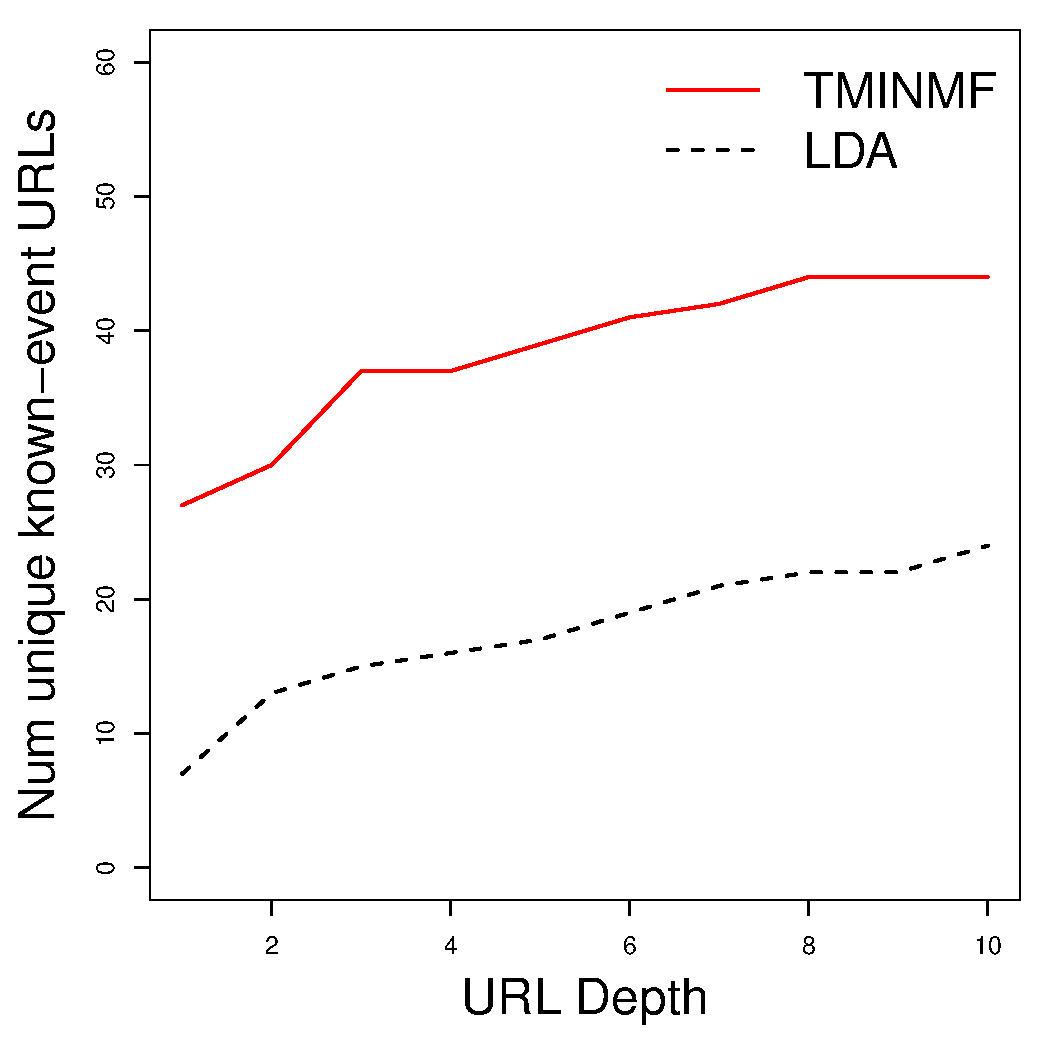
\includegraphics[width=9cm]{plots/events_at_depth.pdf}
\end{subfigure}%
\begin{subfigure}{.5\textwidth}
  \centering
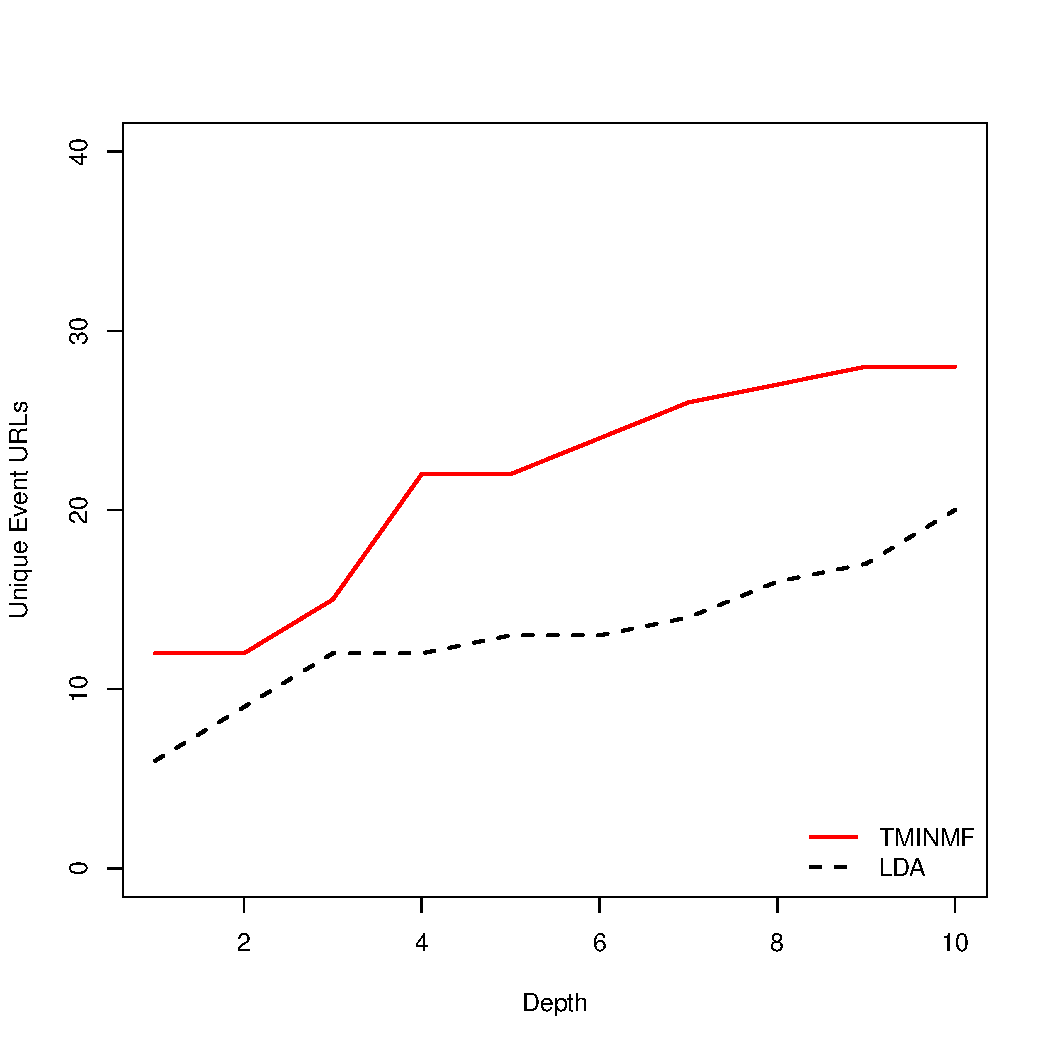
\includegraphics[width=9cm]{plots/unique_urls_at_depth.pdf}
\end{subfigure}
\begin{subfigure}{.5\textwidth}
  \centering
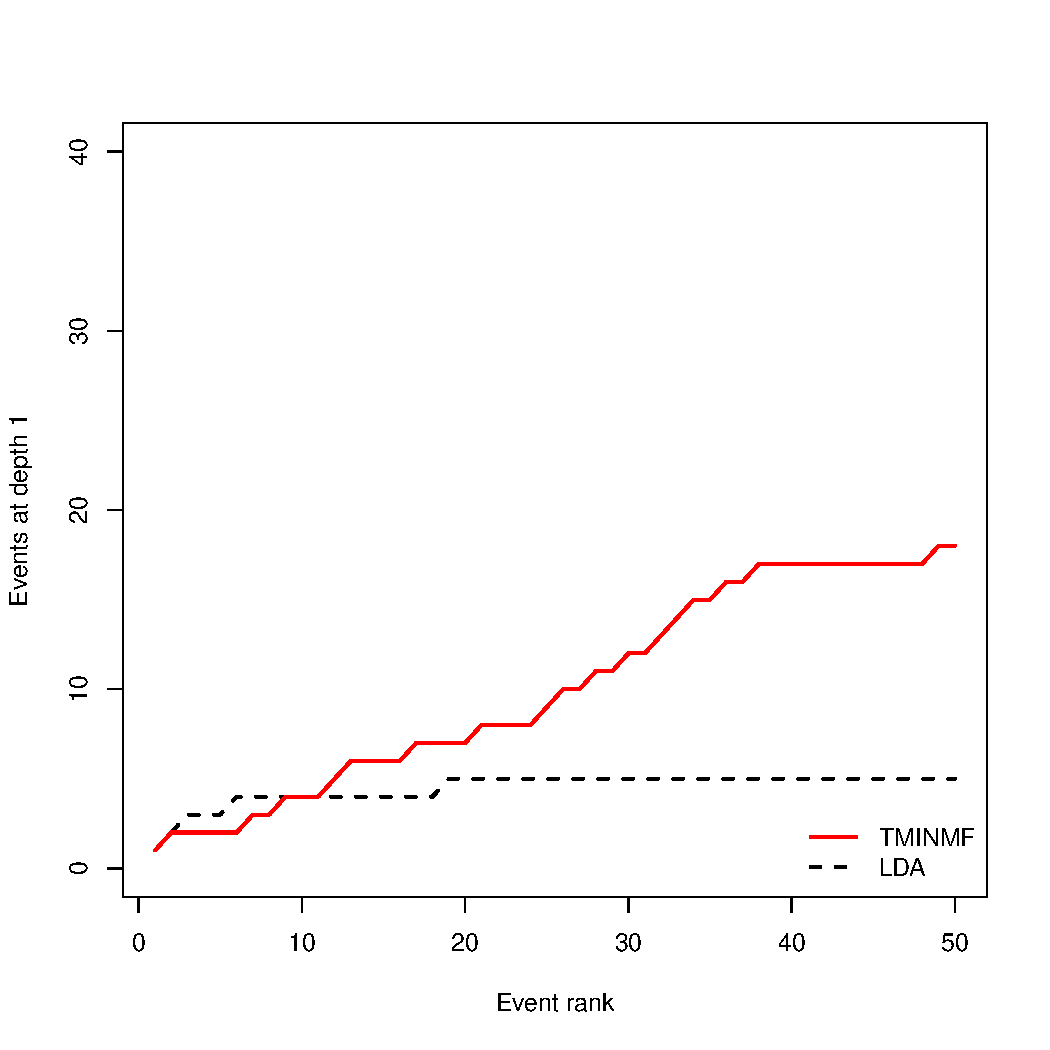
\includegraphics[width=9cm]{plots/events_at_rank_1.pdf}
\end{subfigure}%
\begin{subfigure}{.5\textwidth}
  \centering
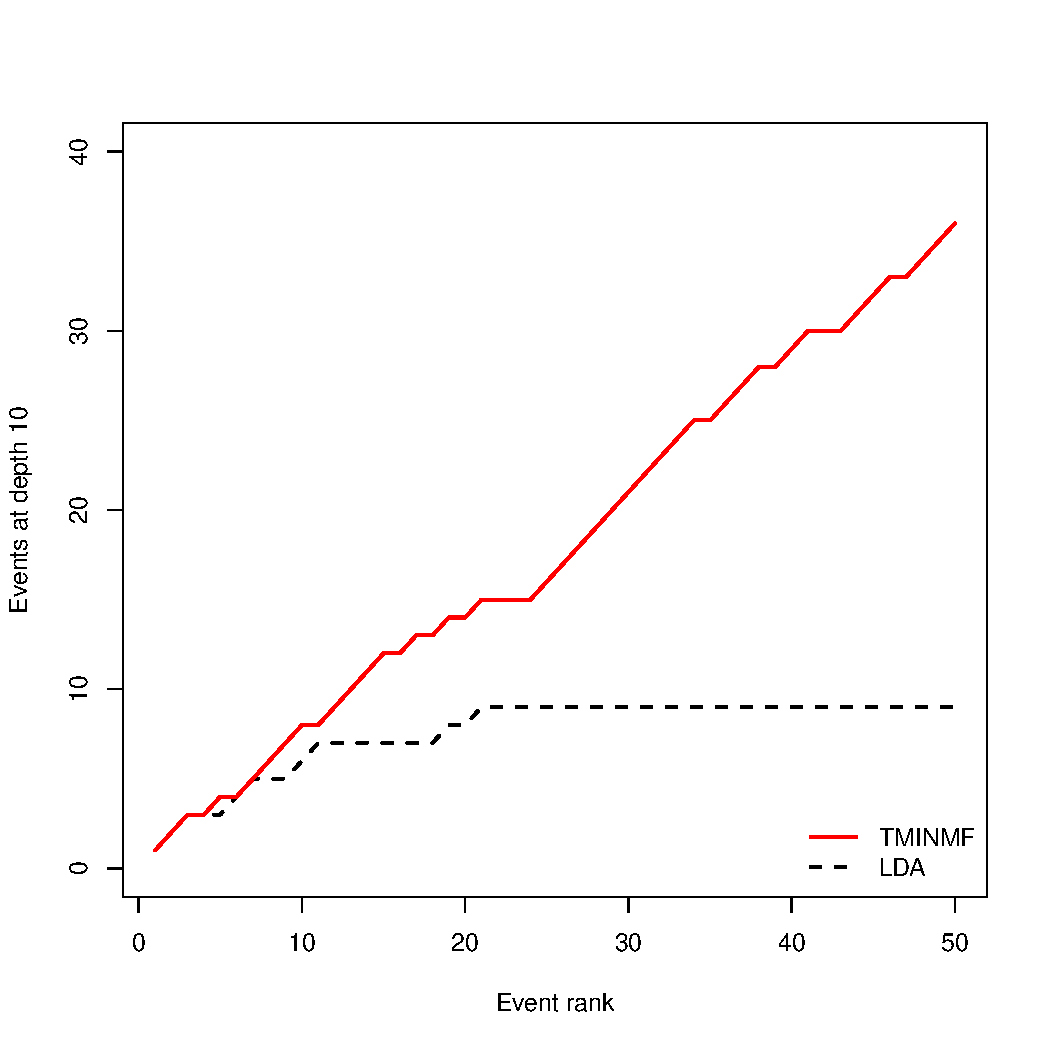
\includegraphics[width=9cm]{plots/events_at_rank_10.pdf}
\end{subfigure}
\caption{(a) number of known-events at each URL depth, (b) number of unique known-event URLs at each depth (c) number of known events at depth 1 for all ranks, (d) number of known events at depth 10 for all ranks.}
\label{fig.eventdist}
\end{figure*}

\begin{table*}
\small
\begin{tabular}{| l | p{7cm} | p{7cm} | } \hline
{\bf ID } & {\bf TMINMF} & {\bf LDA } \\ \hline
1 & wesley(0.075) clark(0.074) dean(0.055) primary(0.052) howard(0.05) edwards(0.05) kerry(0.049) hampshire(0.048) 2004(0.045) missouri(0.044) & 
edwards(0.048) dean(0.048) campaign(0.043) dr(0.034) kerry(0.025) candidate(0.024) s(0.018) iowa(0.018) primary(0.016) clark(0.016) \\ \hline
2 & taguba(0.036) soldier(0.035) detainee(0.03) prisoner(0.029) karpinski(0.029) ricardo(0.028) fay(0.028) maj(0.028) command(0.027) cellblock(0.027) &
prisoner(0.034) military(0.033) abuse(0.026) detainee(0.025) interrogate(0.023) iraq(0.023) prison(0.021) abu(0.018) ghraib(0.018) america(0.013) \\ \hline
3 & poll(0.181) voter(0.131) politics(0.131) bush(0.112) election(0.11) campaign(0.102) vote(0.098) candidate(0.066) senator(0.061) kerry(0.056) &
kerry(0.135) bush(0.071) campaign(0.046) s(0.038) president(0.028) john(0.018) senator(0.016) cheney(0.013) republican(0.012) democrat(0.011) \\ \hline
4 & port(0.044) au(0.04) aristide(0.038) prince(0.033) philippe(0.032) rebel(0.03) haitien(0.028) gona(0.028) politics(0.028) haiti(0.025) &
haiti(0.049) aristide(0.037) government(0.022) cuba(0.018) s(0.015) president(0.014) rebel(0.013) chile(0.013) zimbabwe(0.012) country(0.011) \\ \hline
5 & sadr(0.05) moktada(0.044) baghdad(0.042) sunni(0.039) militia(0.037) falluja(0.036) occupation(0.03) gen(0.027) struggle(0.026) karbala(0.026) &
vote(0.077) election(0.059) voter(0.057) percent(0.03) poll(0.027) ballot(0.022) party(0.021) candidate(0.018) republican(0.016) democratic(0.015) \\ \hline
\end{tabular}
\caption{Top 5 events detected by TMINMF and LDA methods}
\label{table.top5}
\end{table*}




\end{document}
